\documentclass{article}
\usepackage{amsfonts}
\usepackage{amsmath}
\usepackage{amssymb}
\usepackage{graphicx}
\usepackage[font=small, labelfont=bf, justification=centering]{caption}
\usepackage[colorlinks=true, linkcolor=black, urlcolor=red, citecolor=black]{hyperref}
\usepackage[a4paper, margin=1in]{geometry}

\begin{document}
  {\centering \textbf{Problema 1} \par}
  Uma \textit{palavra} é uma sequência de letras maiúsculas do
  nosso alfabeto (isto é, há 26 possíveis letras). Uma palavra é chamada de
  \textit{palíndromo} se tem pelo menos duas letras e ela é a mesma palavra se lida da
  esquerda para a direita ou da direita para a esquerda. Por exemplo, as palavras ARARA
  e NOON são palíndromos, mas BOBO e AÑÃ não são palíndromos.

  Dizemos que uma palavra $x$ \textit{contém} uma palavra $y$ se existem letras
  \textit{consecutivas} de $x$ que juntas formam $y$. Por exemplo, a palavra ARARA
  contém a palavra RARA e também a palavra ARARA, mas não contém a palavra ARRA.

  Calcule a quantidade de palavras de 14 letras que contêm algum palíndromo.

  \medskip

  {\centering \textbf{Resposta} \par}
  Sabe-se que existem \(26^{14}\) possibilidades de palavras de \(14\) letras no total. Além disso, podemos afirmar também que toda palavra contém no mínimo um palíndromo de $2$ ou $3$ letras.
  Isso ocorre porque, ao retirar as primeira e última letras de um palíndromo, será obtido outro palíndromo (caso tenha mais de $2$ letras). É possível repetir isso até chegar
  a $xx$ (um palíndromo de $2$ letras), ou $xyx$ (um palíndromo de $3$ letras).
  
  Existem 26 possíveis letras para a \(1\textsuperscript{a}\) letra de um não palíndromo de 14 totais letras. Afim de evitar um palíndromo, a \(2\textsuperscript{a}\)
  deve ser diferente da \(1\textsuperscript{a}\), (25 opções). Pelo mesmo motivo, a \(3\textsuperscript{a}\) é diferente da \(1\textsuperscript{a}\) e da \(2\textsuperscript{a}\),
  (24 opções). Esse argumento da \(3\textsuperscript{a}\) letra será válido para todas as outras 11 letras. Com isso podemos concluir que existem \(26^{14} - 26 \cdot 25 \cdot 24^{12}\)
  palíndromos no total.


  \noindent\rule{\linewidth}{0.4pt}
  {\centering \textbf{Problema 2} \par}
  Mostre que não existem triplas de inteiros não negativos
  $(x, y, z)$ satisfazendo a equação
  \[
    x^2 = 5^y + 3^z.
  \]
  \medskip

  {\centering \textbf{Resposta} \par}

  Já que \textit{ímpar + ímpar = par}, $5^y + 3^z$ é par, logo $x$ é par. 
  Se $x = 2k$, $x^2 = 4k^2$, logo $x^2 \equiv 0 \pmod{4}$. Neste caso,
  $0 \equiv 5^y + 3^z \equiv 1 + (-1)^z \pmod{4}$, por conseguinte, $z$ é um número
  ímpar. Claramente, $x \not\equiv 0 \pmod{3}$, pois
  \[
    x \equiv 0 \pmod{3} \Rightarrow 5^y = x^2 - 3^z \Rightarrow 5^y \equiv 0 \pmod{3}
  \]
  Absurdo! Agora, nos resta apenas $x \equiv 1 \pmod{3}$ ou $x \equiv 2 \pmod{3}$. Perceba abaixo
  que $x \not\equiv 1 \pmod{3}$ e $x \not\equiv 2 \pmod{3}$, e como já vimos que
  $x \not\equiv 0 \pmod{3}$, não existem soluções para $x$.
  \begin{enumerate}
    \item \textit{Caso 1:} $x \equiv 1 \pmod{3} \Rightarrow x^2 - 5^y = 3^z \Rightarrow y = 2w$. Neste caso, podemos afirmar
      que $x^2 - 5^{2w} = 3^z \Rightarrow (x + 5^w)(x - 5^w) = 3^z$. Para que esta igualdade
      seja verdadeira, ou $x + 5^w \equiv 0 \pmod{3} \quad \text{e} \quad x - 5^w = 1$, ou, tanto
      $x + 5^w$ quanto $x - 5^w$ são múltiplos de 3. Evidentemente $x - 5^w \neq 1$,
      pois se $x - 5^w = 1$, $5^w + 1 \equiv 1 \pmod{3} \Rightarrow 5^w \equiv 0 \pmod{3}$, absurdo!
      Mas é impossível também que tanto $x + 5^w$ quanto $x - 5^w$ sejam múltiplos de 3, pois neste caso,
      $x \equiv 5^w \pmod{3} \Rightarrow  x \equiv 5^w \equiv 1 \pmod{3}$, impossibilitando que
      $x - 5^w \equiv 0 \pmod{3} \therefore x \not\equiv 1 \pmod{n}$
    \item \textit{Caso 2:} $x \equiv 2 \pmod{3} \Rightarrow x^2 \equiv 5^w \equiv 1 \pmod{3}$.
      Evidentemente $x + 5^w \not\equiv 0 \pmod{3}$, logo a única opção é que $x + 5^w = 1$, claramente impossível já
      que tanto $x$ quanto $w$ são números inteiros positivos $\therefore x \not\equiv 2 \pmod{3}$
  \end{enumerate}

  \noindent\rule{\linewidth}{0.4pt}

  {\centering \textbf{Problema 3} \par}

  No triângulo escaleno $ABC$, sejam $I$ o seu incentro e $D$ o
  ponto onde $AI$ intersecta $BC$. Sejam $M$ e $N$ os pontos onde o incírculo de $ABC$
  toca $AB$ e $AC$, respectivamente. Seja $F$ o segundo encontro do circuncírculo $(AMN)$
  com o circuncírculo $(ABC)$. Seja $T$ o encontro de $AF$ com o prolongamento de $BC$.
  Seja $J$ a interseção de $TI$ com a paralela a $FI$ que passa por $D$. Prove que $AJ$ é
  perpendicular a $BC$.

  \textit{Nota: o incentro de um triângulo é a interseção das bissetrizes internas.}

  \begin{figure}[h]
    \centering
    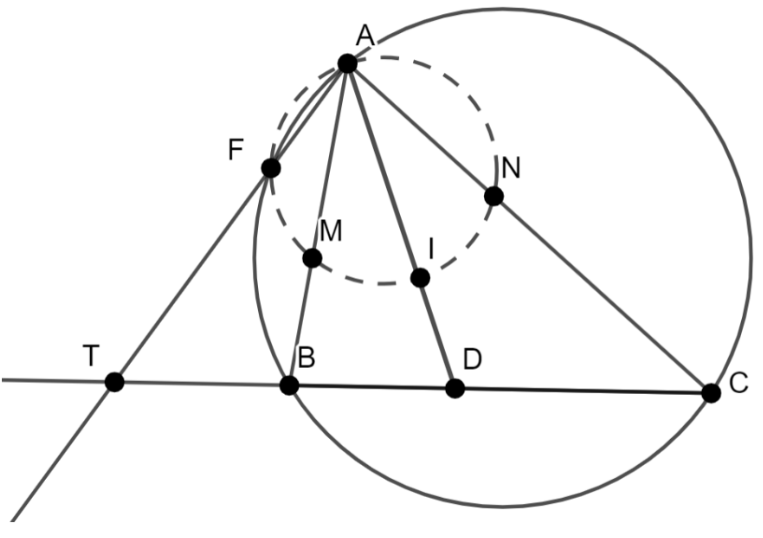
\includegraphics[width=0.5\textwidth]{third.png}
    \caption{Uma ilustração do terceiro problema. \href{https://noic.com.br/wp-content/uploads/2025/03/Solucoes_do_TM2_2024_Nivel_A.pdf}{Fonte}}
  \end{figure}

  \medskip

  {\centering \textbf{Resposta} \par}

  \noindent\rule{\linewidth}{0.4pt}

  {\centering \textbf{Problema 4} \par}
  Encontre todos os inteiros positivos $a$, $b$ e $c$ tais que 
  \[
    3ab = 2c^2 \quad \text{e} \quad a^3 + b^3 + c^3
  \]
  seja o dobro de um número primo.

  \medskip

  {\centering \textbf{Resposta} \par}

\end{document}
